\RequirePackage{ifluatex}
\let\ifluatex\relax

\documentclass[aps,%
12pt,%
final,%
oneside,
onecolumn,%
musixtex, %
superscriptaddress,%
centertags]{article} %% 
\topmargin=-40pt
\textheight=650pt
\usepackage[english,russian]{babel}
\usepackage[utf8]{inputenc}
%всякие настройки по желанию%
\usepackage[colorlinks=true,linkcolor=black,unicode=true]{hyperref}
\usepackage{euscript}
\usepackage{supertabular}
\usepackage[pdftex]{graphicx}
\usepackage{amsthm,amssymb, amsmath}
\usepackage{textcomp}
\usepackage[noend]{algorithmic}
\usepackage[ruled]{algorithm}
\usepackage{lipsum}
\usepackage{indentfirst}
\usepackage{babel}
\usepackage{pgfplots}
\pgfplotsset{compat=1.9}

\pgfplotsset{model/.style = {blue, samples = 100}}
\pgfplotsset{experiment/.style = {red}}

\selectlanguage{russian}

\setlength{\parindent}{2.4em}
\setlength{\parskip}{0.1em}
%\renewcommand{\baselinestretch}{2.0}

\usepackage{xcolor}
\usepackage{hyperref}
 
 % Цвета для гиперссылок
%\definecolor{linkcolor}{HTML}{799B03} % цвет ссылок
%\definecolor{urlcolor}{HTML}{799B03} % цвет гиперссылок
 
%\hypersetup{pdfstartview=FitH,  linkcolor=linkcolor,urlcolor=urlcolor, colorlinks=true}

%\documentclass[aps,%
%12pt,%
%final,%
%oneside,
%onecolumn,%
%musixtex, %
%superscriptaddress,%
%centertags]{article} %% 
%\topmargin=-40pt
%\textheight=650pt
%\usepackage[english,russian]{babel}
%\usepackage[utf8]{inputenc}
%всякие настройки по желанию%
%\usepackage[colorlinks=true,linkcolor=blue,unicode=true]{hyperref}
%\usepackage{euscript}
%\usepackage{supertabular}
%\usepackage[pdftex]{graphicx}
%\usepackage{amsthm,amssymb, amsmath}
%\usepackage{textcomp}
%\usepackage[noend]{algorithmic}
%\usepackage[ruled]{algorithm}
%\selectlanguage{russian}

\begin{document}

\begin{titlepage} 
\begin{center}
% Upper part of the page
%\textbf{\Large САНКТ-ПЕТЕРБУРГСКИЙ ГОСУДАРСТВЕННЫЙ ЭКОНОМИЧЕСКИЙ УНИВЕРСИТЕТ} \\[1.0cm]
%\textbf{\large Кафедра Прикладной Математики и Информатики}\\[3.5cm]
 
% Title
\textbf{}\\[10.0cm]
\textbf{\LARGE Финансовая математика}\\[0.5cm]
\textbf{\Large ПМ-1701} \\[0.2cm]

%supervisor
\begin{center} \large
{Преподаватель:} \\[0.5cm]
\textsc {Чернов Алексей Викторович}\\
{alex\_tche@mail.ru}\\
\end{center}
% \begin{flushright} \large
%\emph{Рецензент:} \\
%д.ф. - м.н., профессор \textsc{Надеемся Нам Помогут}
%\end{flushright}
%\begin{flushright} \large
%\emph{Заведующий кафедрой:} \\
%д.ф. - м.н., профессор \textsc{Не Обмани Себя}
%\end{flushright}
\vfill 

% Bottom of the page
{\large {Санкт-Петербург}} \par
{\large {2020 г., 6 семестр}}
\end{center} 
\end{titlepage}

% Table of contents
\begin{thebibliography}{3}
	\bibitem{Sulsky1994}
	Sulsky D., Chen Z., Schreyer H. L.  A particle method for history-dependent materials // Computer Methods in Applied Mechanics and Engineering. --- 1994, V. 118. --- P. 179--196.
	\bibitem{LiuLiu}
	Liu G. R., Liu M. B. Smoothed particle hydrodynamics: a meshfree particle method. --- Singapore : World Scientific Publishing. --- 2003. --- 449 p.
\end{thebibliography}
\tableofcontents
\newpage
\section{Конспекты лекций}
\subsection{ Простая и сложная процентная ставка 05.02.2020} 

Для иллюстрации понимания работы сложного и простого процента введем следующие обозначения:
\begin{itemize} 
  \item $i$ - процентная ставка (по умолчанию годовая)
  \item $t$ - срок вклада
  \item $S_{0} = P$ - начальный вклад
  \item \textbf{$S$} - конечный вклад
  
\end{itemize}

Опр: \textit{Простыми процентами} называются такие процентные ставки, которые применяются к одной и той же первоначальной сумме на протяжении всей финансовой операции

Опр: \textit{Сложными процентами} называются ставки, применяемые после каждого интервала начисления к сумме первоначального долга и начисленных за предыдущие интервалы процентов.
\label{first_table}
\begin{table}[H]
	\begin{center}
		\begin{tabular}{c|c|c} 
		t (год) & Простой процент (\%) & Сложный процент (\%) \\ \hline
		0 & \textbf{100} & 100  \\ 
		1 & \textbf{110} & 110 \\ 
		2 & \textbf{120} & 121
		\end{tabular}
	\caption{Пример использования сложных и простых процентов}
	\end{center}
\end{table}
\subsubsection{Формулы простых процентов}
Формула для $S_{n+1}$: $$S_{n+1}=S_n+S_0\cdot i  $$

Формула для конечного вклада: $$S=P+P\cdot i\cdot n=P\cdot (1+i\cdot n) $$

Формула для начального вклада: $$P=\frac{S}{1+i\cdot n} $$

Формула для процентной ставки: $$i=\frac{\frac{S}{P}-1}{t}=\frac{S-P}{t\cdot P}$$

Формула для продолжительности вклада: $$ t=\frac{\frac{S}{P}-1}{i}=\frac{S-P}{i\cdot P}$$

\subsubsection{Формулы простых процентов}
Формула для $S_{n+1}$: $$S_{n+1}=S_n\cdot (1+i) = S_n + S_n\cdot i  $$

Формула для конечного вклада: $$S = P\cdot (1+i)^n $$

Формула для начального вклада: $$P=\frac{S}{(1+i)^n} $$

Формула для процентной ставки: $$i=\sqrt[t]{\frac{S}{P}}-1$$

Формула для продолжительности вклада: $$ t=log_{(1+i)} \frac{S}{P}$$

\subsubsection{Срок удвоения вклада}

\textbf {Для простого процента:} 
$$2P=P\cdot(1+i\cdot t_{new})$$ 
$$t_{new}=\frac{1}{i}$$

\textbf {Для сложного процента:} 
$$2P=P\cdot(1+i)^{t_{new}}$$ 
$$2 = (1+i)^{t_{new}}$$ 
$$t_{new}=log_{(1+i)} 2 $$

\subsubsection{Задача о.в Манхэттен}
\label{second_table}
\begin{table}[H]
	\begin{center}
		\begin{tabular}{c|c} 
		t (год) & Деньги (\$) \\ \hline
		$t_1$ - 1626 год & $P - 24$ \\ \hline
		$t_2$ - 2019 год & $S - 49\cdot 10^9$
		\end{tabular}
		\caption{Данные о Манхэттене}
	\end{center}
\end{table}

\textbf{Вопрос}: Какова процентная ставка при простом и сложном проценте?

\textbf{Решение:}

Простой процент: 
$$i=\frac{\frac{S}{P}-1}{t}=\frac{S-P}{(t_2-t_1)\cdot P}=\frac{49\cdot 10^9-24}{24*(2019-1626)}=5.19 \cdot 10^6$$

Сложный процент: 
$$i=\sqrt[(t_2-t_1)]{\frac{S}{P}}-1=\sqrt[2019-1626]{\frac{49\cdot 10^9}{24}}-1 = 0.056 = 5.6\%$$

Срок удвоения оклада: 
$$t_{new}=log_{(1+i)} 2 = log_{(1+0.056)} 2 = 12.7 \approx 13 \text{ years}$$ 

\subsubsection{Смешанная ставка}

Опр: \textit{Смешанная процентная ставка} - ставка, которая осуществляется по следующему правилу - в пределах года используется простая ставка, а остальные - по сложной.

Формула для смешанной процентной ставки:
$$S = P\cdot (1+i_c)^{[t]} + P\cdot (1+i_c)^{[t]} \cdot {\{t\}}\cdot i_p = P(1+i_c)^{[t]} \cdot (1 + {\{t\}}\cdot i_p ) $$
где ${[t]}$ - целая часть числа, а  ${\{t\}}$ - дробная.
\begin{figure}[h!]
	
	\begin{center}
	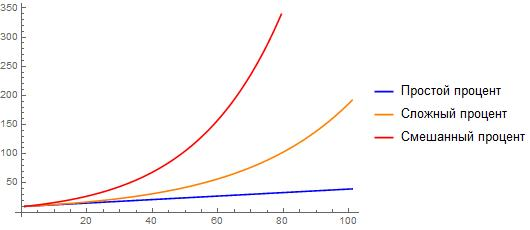
\includegraphics[scale=0.6]{images/first.jpg}
	\caption{График простой, сложной и процентной ставки}
	\end{center}
\end{figure}
\newpage


\subsection{Процентная ставка для разных периодов времени 09.02.2020 }

Пусть задана простая процентная ставка. Нужно найти эквивалентную месячную ставку.
$$ P\cdot (1+i_{year} \cdot t) = P \cdot (1+12 \cdot i_{m}\cdot t) $$
$$i_{m} = \frac{i_{year}}{12} $$
$$i_{d} = \frac{i_{year}}{365} $$

Такой способ приведения и соотношения называются \textit{относительными}.

Для сложных процентов:
$$ S = P\cdot (1+i_{year})^n  = P\cdot (1+i_{m})^{12n} $$
$$ i_{m} = \sqrt[12]{1 + i_{year}} - 1 $$

А такой способ называется \textit{уравновешенным}.

Пример:

Банк предъявляет простую годовую ставку $i_{year}$ на срок до $3$-х лет. Можем ли мы придумать более легкую стратегию? Да, мы можем положить деньги на вклад, снять деньги, а потом заново открыть вклад. Рассмотрим решение задачи двумя разными способами:

\textbf{Решение:}

$$ P \cdot (1+i \cdot t) < P (1+i)^t $$

Если использовать месячную ставку, то получаем формулу:

$$(1+\frac{i}{12})^{12} = {Binom Newion} = 1 + 12 \frac{i}{12} + ... + > (1+i) $$
$$ i>0 \text{, } t > 1 $$
$$ \lim_{m\to \infty} (1+\frac{i}{m})^{t\cdot m} = \lim_{m\to \infty} ((1+\frac{i}{m})^{\frac{m}{i}})^{t\cdot i} = e^{it} $$

Такое начисление процентов называется \textit{непрерывным}.

$$ S = P \cdot e^{it} $$

Для сложной процентной ставки:
$$ S = P \cdot (1+i)^t = P \cdot e^{\alpha \cdot t} $$
$$ \alpha = \ln (1+i) $$

$\alpha$ - сила роста, сила процента, скорость относительного прироста вклада за $\Delta t \rightarrow 0$

$$ \frac{\Delta f}{f \Delta t} = \frac{f'}{f} $$

$$S(t) = P \cdot e^{\alpha \cdot t}$$

Высчитаем силу прироста для функции $S(t)$
$$ \frac{S'}{S} = \frac{P \cdot e^{\alpha \cdot t} \cdot \alpha}{P \cdot e^{\alpha \cdot t}} = \alpha $$

\subsubsection{Переменная процентная ставка}

Пусть на каком-то интервале времени $t_1$ действовала ставка $i_1$, на каком-то другом времени $t_2$ выполнялась ставка $t_2$ и.т.д. Ставка была простая, процентны набегали только на начальный вклад.

Задача: найти эквивалентную среднюю процентную ставку, которая по формуле простой процентной ставки приводила к такому же результату. 

\begin{center}
	\begin{tikzpicture}
		\begin{axis}[xmin = 1, legend pos = north west, scale = 1, xmax = 5,title=График переменной процентной ставки, grid = major]
		\addplot [model] {-5+35*x};
		\addplot [scatter]coordinates { (1,30) (2,50) (3,80) (4,120) (5,170)} ;
		\end{axis}
	\end{tikzpicture}
\end{center}
$$ T =  \sum_{i}{\tau_i} $$

Формула для конечного вклада при переменной ставке для простых процентов:
$$ P = P \cdot (1+\tau_1 \cdot i_1 + \tau_2 \cdot i_2 + ... + \tau_n \cdot i_n) = P \cdot (1+ \overline{i}\cdot T) $$

Обозначим за $ k_j = \frac{\tau_j}{T}$. Также очевидно, что $\sum k_j = 1$

Формула для средней ставке процентов при переменной ставке для простых процентов.
$$ \overline{i} = \sum_{k}{k_j\cdot i_j} $$

Для переменной процентной сложной ставки выведем похожую формулу:
$$ P \cdot (1+i_1)^{t_1} \cdot (1+i_2)^{t_2} \ldots (1+i_n)^{t_n} =P \cdot  (1+\overline{i})^{T} $$
$$ T =  \sum_{i}{\tau_i} $$

Обозначим за $ k_j = \frac{\tau_j}{T}$. Также очевидно, что $\sum k_j = 1$.
Формула для средней ставки сложных процентов равна:
$$ \overline{i} = \prod_j (1+i_j)^{\tau_j}  - 1 $$
\end{document}